\newprob{1718343693}
{
    在一個半徑為$r$的環上共有$+q$ 電荷,平均分佈 在表面。如果環以角速度$\omega$ 轉動,環上所產生 的電流是多少?\zzh{3}
    \par{\par\centering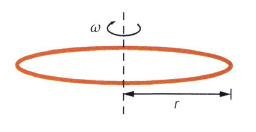
\includegraphics[width=.35\textwidth]{./img/ch2_circuit_lq_2024-06-14-14-33-19.png}\par}

}{
    \par{\par\centering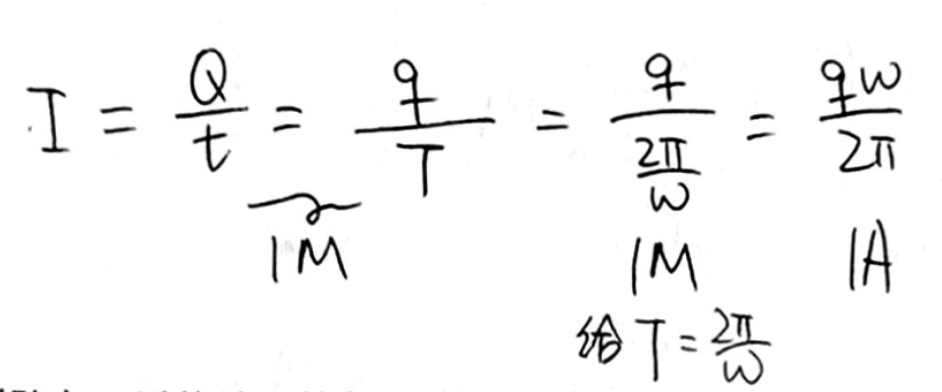
\includegraphics[width=.7\textwidth]{./img/ch2_circuit_lq_2024-06-15-15-15-11.png}\par}
}
% surround all number+units with \qty{number}{units}, and then make all letters (e´.g. A, BB, ACDEG, r, i, x) into math mode $$
\newprob{1718344747}
{
    電路在$G$點接地。若有\ qty{2}{C}電荷流經路徑$ACDEB$上,經過$CD$後,它們失去 \qty{4}{J}電能。經過$DE$後,它們失去 \qty{10}{J}電能。求電源的電動勢,並直接寫出圖中各點的勢。(提示:接地處電勢為 \qty{0}{V})\par\zzh{3}
    \par{\par\centering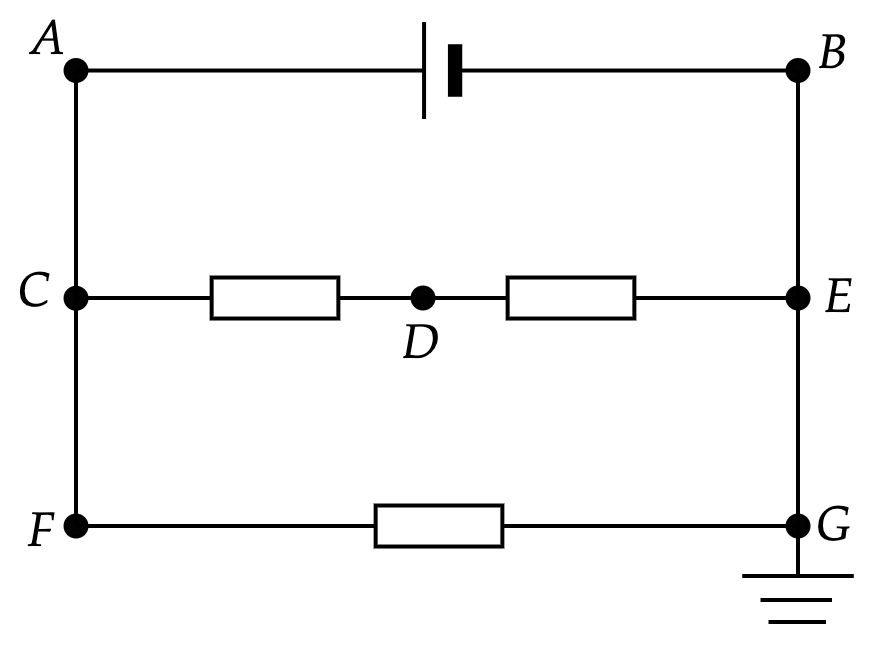
\includegraphics[width=.4\textwidth]{./img/ch2_circuit_lq_2024-06-14-13-59-11.png}\par}
}{
    \begin{itemize}
        \item [] $V_{CD}=\dfrac{W}{Q}=4/2=\qty{2}{V}$
        \item[]  $V_{DE}=\dfrac{W}{Q}=10/2=\qty{5}{V}$\giveM
        \item [] $\varepsilon=V_{CD}+V_{DE}=2+5=\qty{7}{V}$\giveM
        \item [] 電勢:$A, C, F=\qty{7}{V}$,$D=\qty{5}{V}$,$B, E, G=\qty{0}{V}$\giveA
    \end{itemize}
}

\newprob{1718345256}
{
    圖中固定電阻器 的電阻是 \qty{10}{\ohm},電池組電動勢為 \qty{6}{V}。變阻器電阻值 範圍為0 - \qty{60}{\ohm}。滑動觸點在位置$X$上,且$AX=\frac{5}{6}AB$。求伏特計的讀數。\zzh{3}
    \par{\par\centering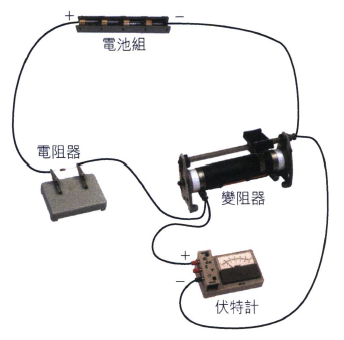
\includegraphics[width=.35\textwidth]{./img/ch2_circuit_lq_2024-06-14-14-10-27.png}\par}
}{
    \begin{itemize}
        \item[] 變阻器接入電路部分的電阻值$R_1=\dfrac{BX}{AB}\times 60$
        \item[]  $=(1-\frac{5}{6})\times 60$
        \item [] $= \qty{10}{\ohm}$\giveM
        \item[]  $I=\dfrac{V'}{R_1+R_2}=\dfrac{6}{10+10}=\qty{0.3}{A}$\giveM
        \item[]  $V=IR_2=0.3\times 10=\qty{3}{V}$\giveA
    \end{itemize}

}


\newprob{1718345442}
{
    % Active physics p122 q11
    有三枚電阻為$R$的電阻器如下圖接駁至電阻為 $3R$ 的電阻線。整個電路的等效電阻是多少?答案以$R$表示。\zzh{3}
    \par{\par\centering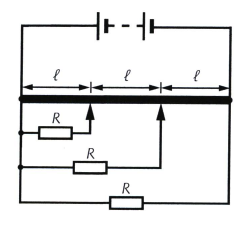
\includegraphics[width=.35\textwidth]{./img/ch2_circuit_lq_2024-06-14-14-12-24.png}\par}

}{
    \src{Active physics p122 q11}
    \par{\par\centering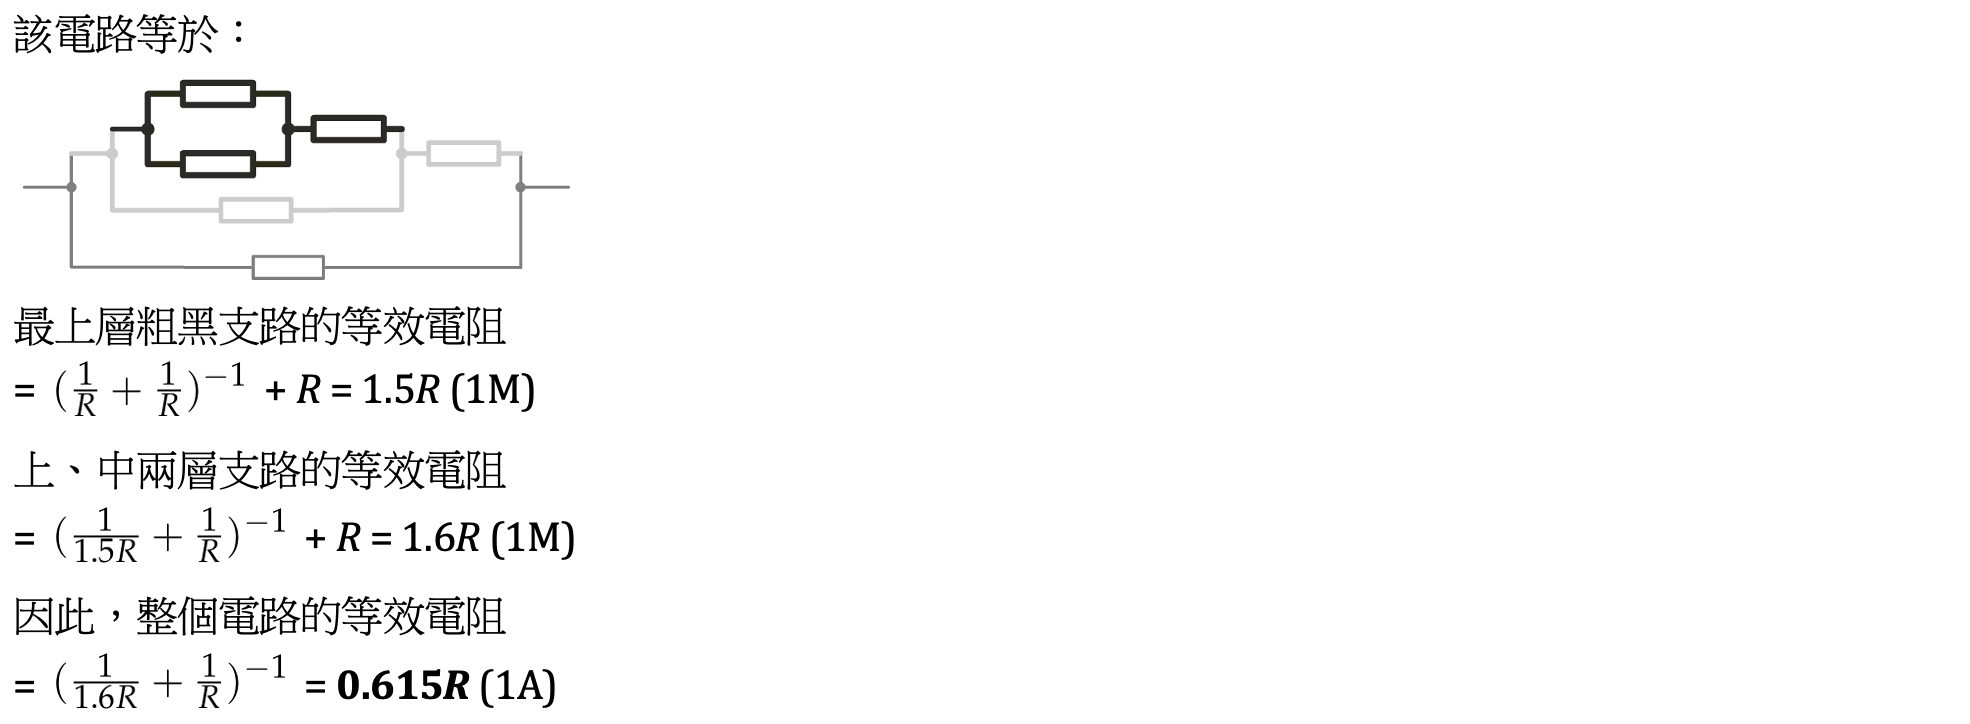
\includegraphics[width=\textwidth]{./img/ch2_circuit_lq_2024-06-16-12-13-04.png}\par}

}

\newprob{1718345588}
{
    % Active physics p122 q13
    如下圖所示,四個相同而電阻皆為R的電阻器 連接至電池。如果流經 X 點的電流為1.0A,流 出電池的電流是多少?
    \zzh{3}
    \par{\par\centering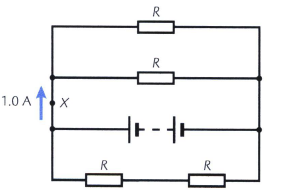
\includegraphics[width=.35\textwidth]{./img/ch2_circuit_lq_2024-06-14-14-13-12.png}\par}
}{
    \src{Active physics p122 q13}
    \par{\par\centering
\includegraphics[width=\textwidth]{./img/ch2_circuit_lq_2024-06-16-12-13-41.png}\par}
}


\newprob{1718345691}
{
    % Active physics p122 q16
    家輝把電池組和電阻器串聯一個熱敏電阻。熱敏 電阻是一種電阻值隨環境温度$T$變化的裝置,如 圖所示。
    \par{\par\centering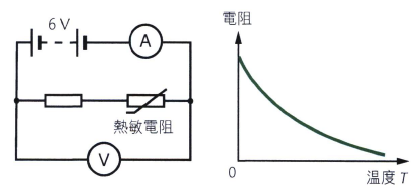
\includegraphics[width=.5\textwidth]{./img/ch2_circuit_lq_2024-06-14-14-15-33.png}\par}
    \begin{parts}
        \part 以下哪一個線圖說明安培計讀數/如何隨温 度$T$而變化?試扼要解釋。\zzh{2}
        \begin{tasks}(2)
            \task \topalign{\par\centering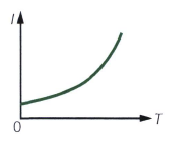
\includegraphics[width=.25\textwidth]{./img/ch2_circuit_lq_2024-06-14-14-16-58.png}\par}
            \task \topalign{\par\centering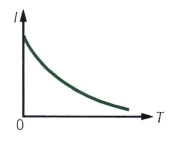
\includegraphics[width=.25\textwidth]{./img/ch2_circuit_lq_2024-06-14-14-17-06.png}\par}
        \end{tasks}
        \part 以下哪一個線圖說明伏特計讀數 $V$ 如何隨温 度$T$而變化?試扼要解釋。\zzh{2}
        \begin{tasks}(2)
            \task \topalign{\par\centering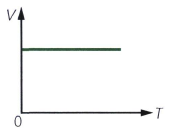
\includegraphics[width=.25\textwidth]{./img/ch2_circuit_lq_2024-06-14-14-17-36.png}\par}
            \task \topalign{\par\centering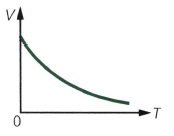
\includegraphics[width=.25\textwidth]{./img/ch2_circuit_lq_2024-06-14-14-17-42.png}\par}
        \end{tasks}


    \end{parts}
}{
    \src{Active physics p122 q16}
    \par{\par\centering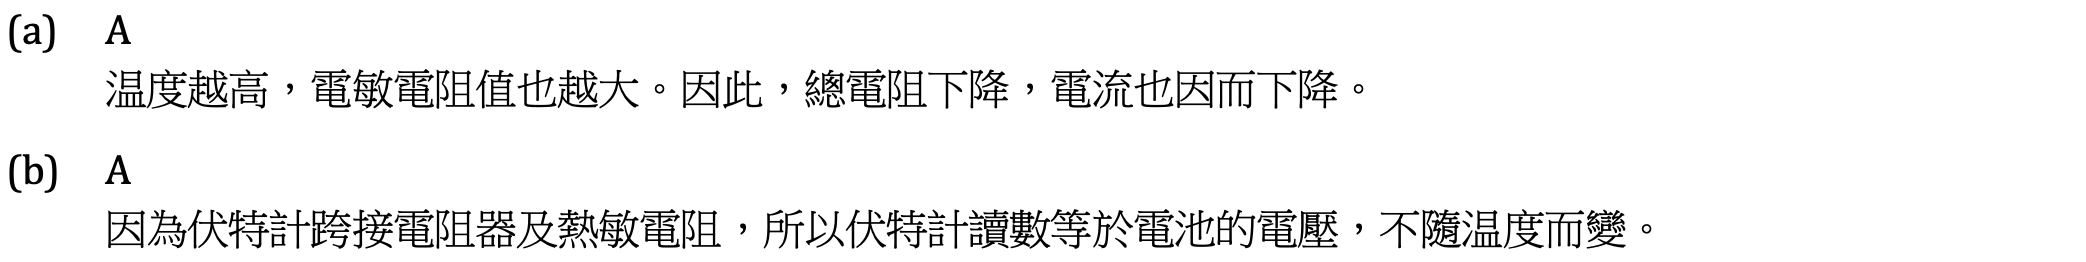
\includegraphics[width=\textwidth]{./img/ch2_circuit_lq_2024-06-16-12-14-26.png}\par}
}

\newprob{1718346030}
{
    % Active physics p131 q10
    如圖 $a$所示,燈泡$X$和$Y$以串聯方式連接至 \qty{32}{V}電池組去。圖$b$顯示燈泡的$I-V$ 特徵曲線。
    \qty{2}{C}
    \par{\par\centering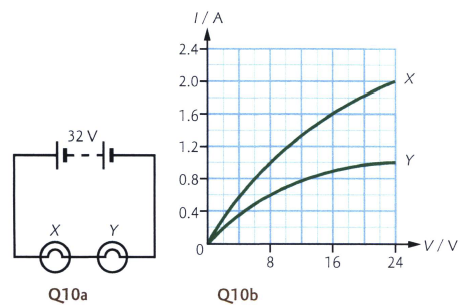
\includegraphics[width=.5\textwidth]{./img/ch2_circuit_lq_2024-06-14-14-21-43.png}\par}
    \begin{parts}
        \part 哪個燈泡較暗?試扼要解釋。\zzh{2}
        \part 找出($a$)部燈泡的電功率。\zzh{2}
    \end{parts}
}{
    \src{Active physics p131 q10}
    \par{\par\centering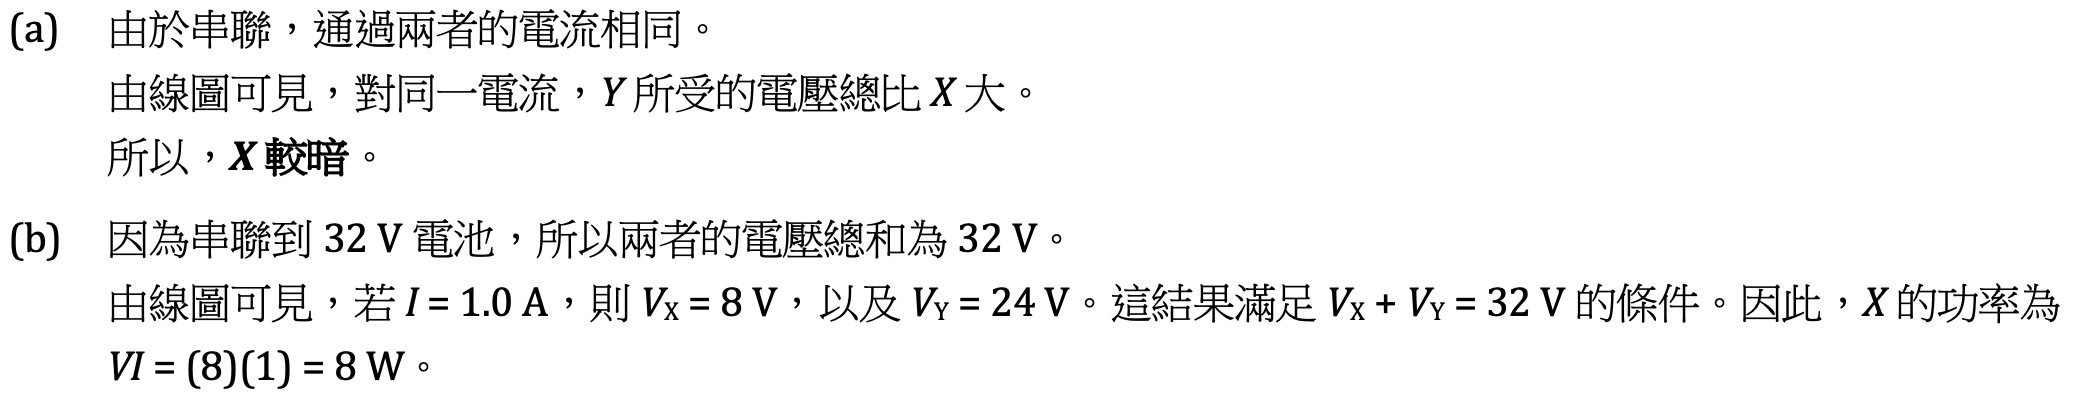
\includegraphics[width=\textwidth]{./img/ch2_circuit_lq_2024-06-16-12-14-51.png}\par}

}

\newprob{1718346191}
{
    % Active physics p138 q9
    以下電路中的伏特計為理想伏特計。
    \par{\par\centering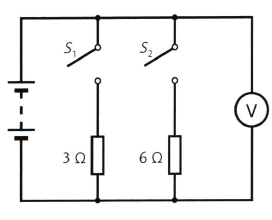
\includegraphics[width=.35\textwidth]{./img/ch2_circuit_lq_2024-06-14-14-23-50.png}\par}
    當$S_1$閉合而$S_2$斷開時,伏特計的讀數為 \qty{12}{V}。 當 $S_2$閉合而$S_1$斷開時,伏特計的讀數為 \qty{16}{V}。

    \begin{parts}
        \part 電池的電動勢$\varepsilon$及內電阻$r$是多少?\zzh{2}
        \part 如果兩個開關同時閉合,伏特計的讀數是多少?\zzh{2}
    \end{parts}
}{
    \src{Active physics p138 q9}
    \par{\par\centering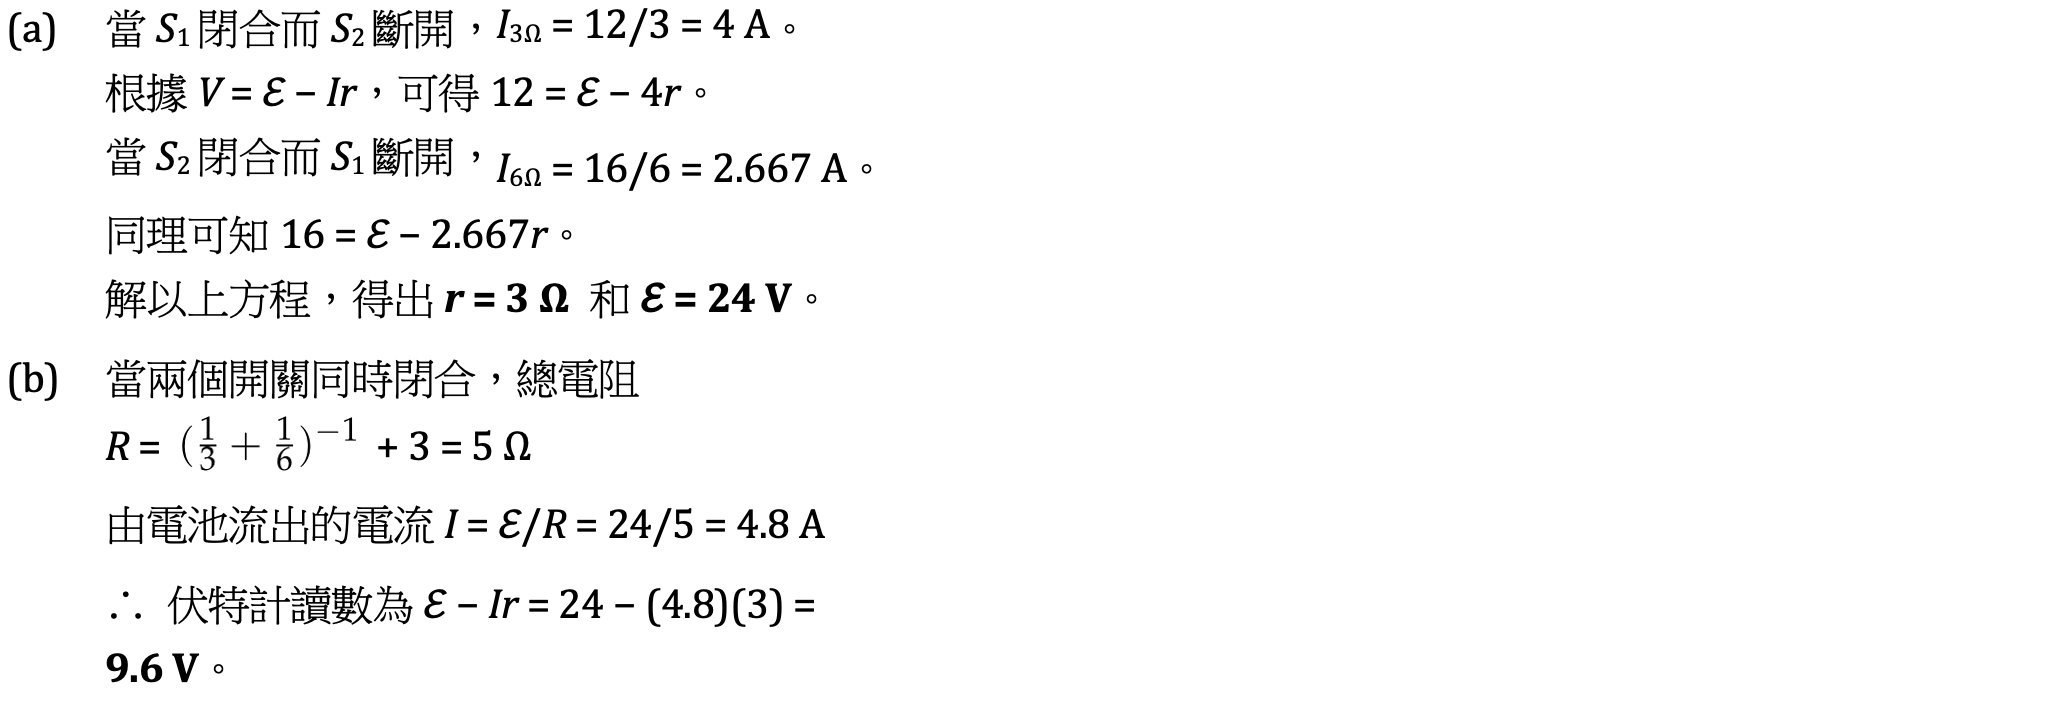
\includegraphics[width=\textwidth]{./img/ch2_circuit_lq_2024-06-16-12-15-17.png}\par}
}